\section{Foundational Concepts}
\label{sec:concepts}

\rx is an adaptive, artificial intelligence based controller and
provides general framework for building reasoning systems for
real-world autonomous vehicles. At MBARI \rx is used for AUV control;
another instantiation of the system is being used for control of a
terrestrial personal robot \cite{pr2, Meeussen:2010dn}. The
development of \rx has been targeted at surveying a number of
oceanographic features which are dynamic and spatio-temporally
unpredictable. Typically this requires our AUVs to balance the goals
of coverage spatially while opportunistically following features of
scientific interest and to do so while being aware of its own
limitations in terms of resources (\eg the battery state of charge)
and overall proximity to other observational assets for obtaining
scientific ground-truth. We are interested in representational
frameworks that allow robots to pursue long-term objectives while
choosing short-term gain and can gracefully deal with exogenous or
endogenous change.

To enable this responsiveness to external observations, the agent has
to be able to synthesize plans insitu and to re-plan without human
intervention. To do so we use a temporal constraint-based planner with
a demonstrated legacy of having flown on NASA space missions. Our
autonomy architecture brings three key innovations for AUV control:
in-situ plan synthesis, the use of flexible plan representations with
a sound theoretical basis and systematic compositional control with
the use of partitioned networks doing so with a demonstrated
capability at sea in novel ocean observation methods.

The next few sections will cover \eu in a bottom-up fashion, going
from the generic theoretical framework that underlies \eue, to the
specific representation, modeling and algorithms implemented by it.  A
brief introduction to Constraint Programming and Constraint-Based
Planning is provided followed by the specific representation that \eu
uses to undertake Constraint-Based Planning.  Subsequently, we provide
an overview of \eus architecture and how it can be embedded in a
planning application such as \rxe. Finally, \eus modeling, inference
and search mechanisms are covered in detail so that the reader can
understand how \rx can perform deliberative planning and react to
execution events by embedding and customizing \eu.

\subsection{Automated Planning}
\label{sec:planningfound}

{\scriptsize
  \begin{quote}
[Planning] \emph{is an abstract, explicit deliberation process that chooses and
organizes actions by anticipating their expected outcomes. This
deliberation aims at achieving as best as possible some prestated
objectives. Automated planning is an area of Artificial Intelligence
(AI) that studies this deliberation process computationally.} -- from
\textbf{Automated Planning Theory and Practice} by Ghallab, Nau and
Traverso \cite{ghallab04} 
\end{quote}
}

\begin{figure} \centering
  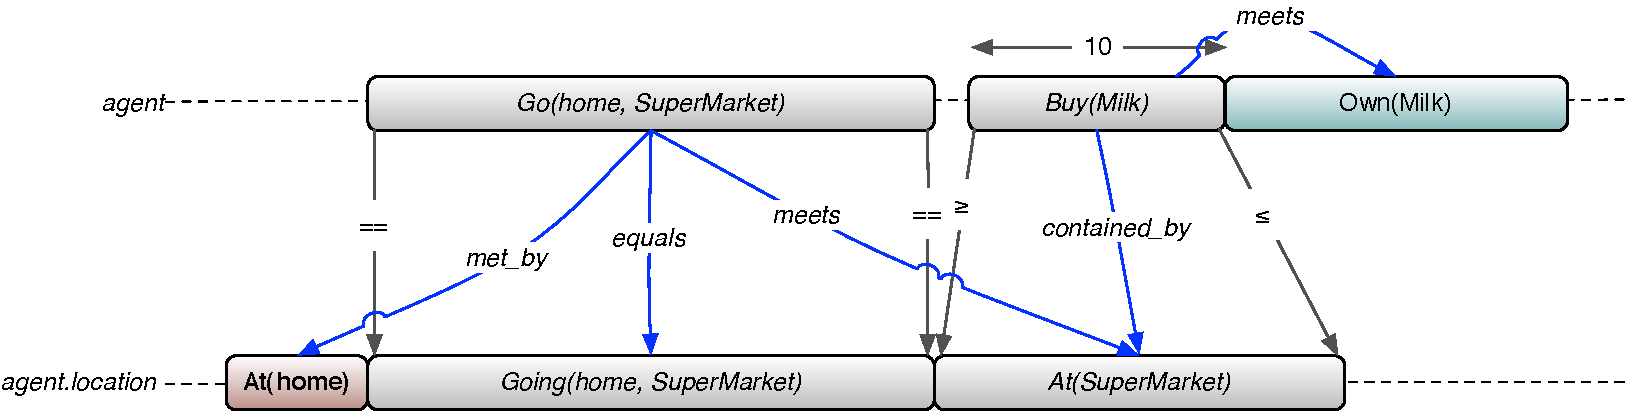
\includegraphics[scale=0.35]{figs/shopping_europa.pdf}
  \caption{\small A potential plan for a robot shopping for groceries.}
\label{fig:shop:shopping}
\end{figure}

To articulate the fundamentals of automated planning briefly and use
that to motivate the mechanisms we use in our specific form of
planning we start with an example.

{\small
  \begin{quote}
    In the near future, a personal robot sets out to buy a gallon of
    milk This involves a number of tasks: obtain keys, obtain wallet,
    start car, drive to store, find and obtain milk, purchase milk,
    etc.  The embedded planner has to have a ``model'' of the world in
    which it lives and has to use the task primitives in this model to
    structure the actions so it achieves its goal. Constraints control
    when certain tasks can or cannot occur. For example the robot must
    obtain the keys and wallet \emph{before} driving to the store and
    pick up the milk \emph{before} purchasing it.
\end{quote}

For such a robot the milk buying plan at the store might look like
that shown in Fig. \ref{fig:shop:shopping}.

At the core of the \rx framework, is the deliberation engine, \eue,
which has a rich legacy from NASA missions \cite{mus98,rajan00,
  jonsson00,aichang04, bresina05}. \eu is a versatile Constraint-based
Temporal Planner which continues to be deployed on a diverse set of
applications including recently, planning for the International Space
Station \cite{barreiro09}. We motivate this section with some problem
domains this planner can handle and then proceed to go into detail.

\paragraph{} {\em Constraint Satisfaction}: A canonical problem in
dealing with constraints is the $N$-Queens problem in which chess queens
must be placed on an  $N \times N$ chessboard so no queens attack the other. % Fig.
% \ref{fig:nqueens-1} shows an example of a random positioning of queens
% on a  $N$x$N$ chessboard. Queens in violation of the non-attack constraint
% are highlighted in red.
% \begin{figure} \centering
%   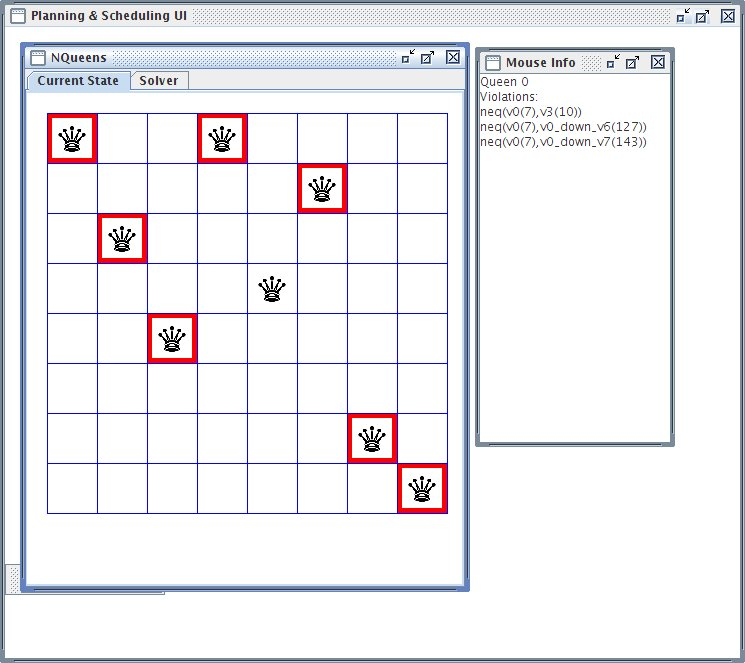
\includegraphics[scale=0.35]{figs/Example-NQueens0.jpg}
%   \caption{\small N-Queens problem. Queens in violation of the
%     non-attack constraint are highlighted in red.}
% \label{fig:nqueens-1}
% \vskip+0.1cm
% \end{figure}
If we define $N$x$N$ variables Q$_{rc}$, $r \in [1,N]$, $c \in [1,N]$,
Q$_{rc} = 1$ if cell $r,c$ in the chessboard is occupied by a Queen,
$0$ otherwise. Then the following constraints need to be satisfied:

\begin{eqnarray*}
 Sum(Q_{rc}) & = & \left\{
   \begin{array}{l l}
     1 & \forall r \quad \mbox{(only one Queen per row)}\\
     1 & \forall c \quad \mbox{(only one Queen per column)}\\ 
   \end{array} \right. \\
Sum(Q_{r+i,c+i}) & = & 1\\
Sum(Q_{r-i,c-i}) & = & 1 \qquad \mbox{(only one Queen on each diagonal)}\\
\end{eqnarray*} 

The problem can be solved by finding assignments for all variables
Q$_{rc}$ that satisfy the above constraints. Fig. \ref{fig:nqueens-2}
is a solution found by \eu using a compact version of that formulation
and a specialized search procedure.

\begin{figure}
\centering
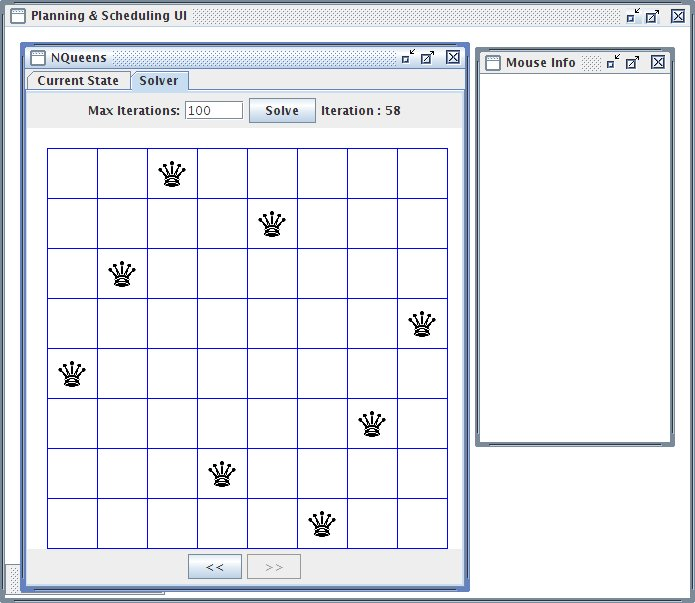
\includegraphics[scale=0.35]{figs/Example-NQueens1.jpg}
\caption{\small $N$-Queens solution generated by \eu}
\label{fig:nqueens-2}
\end{figure}


\paragraph{} \textit{Scheduling}: In the Resource Constrained Project
Scheduling Problem (\texttt{RCPSP}) \cite{Bruckera99}, a project
consisting of a set of activities must be scheduled in a way that
satisfies minimum and/or maximum temporal separation constraints. The
activity schedule must also respect fixed limits on the availability
of resources required to perform each activity. In addition to
satisfying temporal and resource constraints, it is common for the
user to want to minimize makespan \cite{ghallab04} so that the entire
project is finished as early as possible. Fig. \ref{fig:rcpsp-1} shows
an example of a a solution provided by \eu for an \texttt{RCPSP}
instance with 10 activities, 5 resources and 30 temporal constraints.

\begin{figure}
\centering
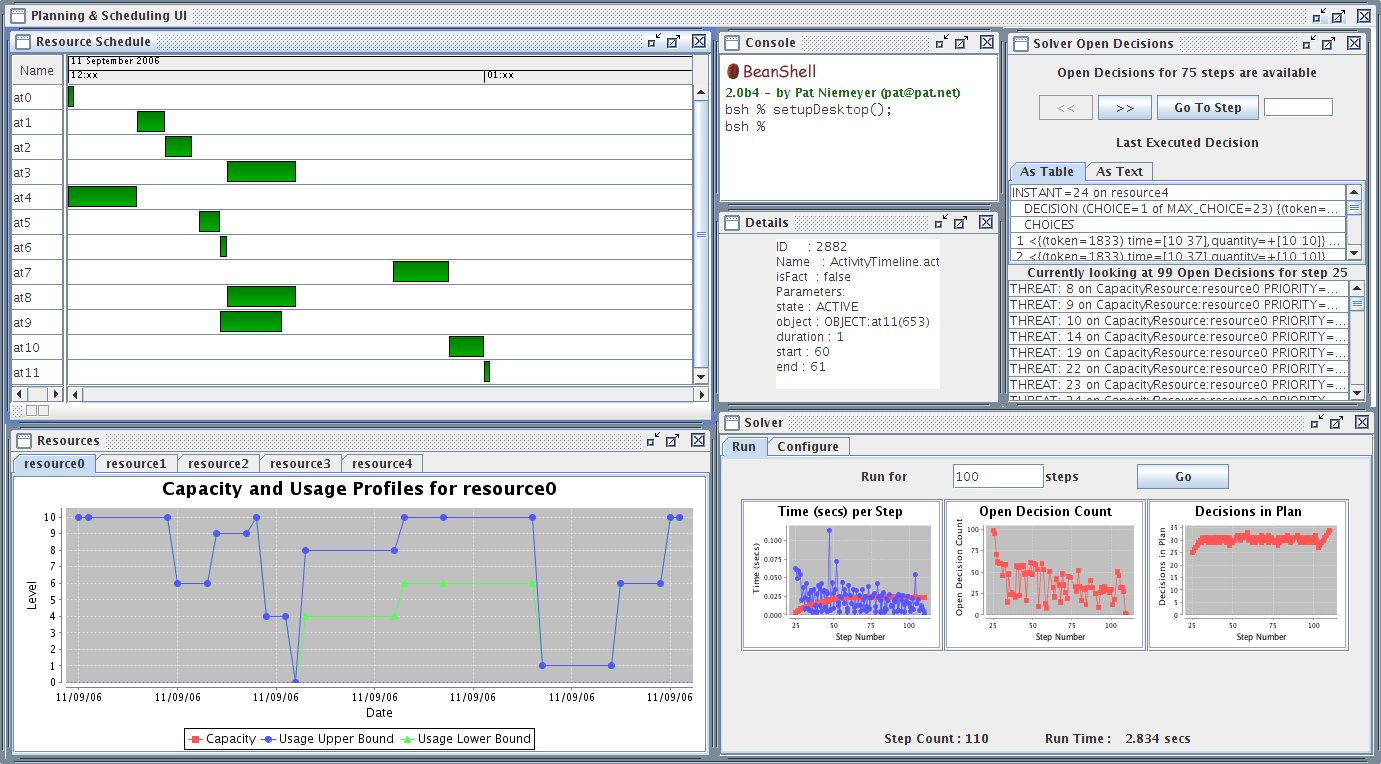
\includegraphics[scale=0.25]{figs/Example-UBO0.jpg}
\caption{\small A \eu solution to an \texttt{RCPSP} \cite{Bruckera99}
  problem.}
\label{fig:rcpsp-1}
\end{figure}


\paragraph{} \textit{Planning}: The Shopping Agent Problem
\cite{russelnorvig} is a variation of the problem with which we
started this chapter.  In this problem, an agent needs to purchase a
set of products (milk, drill, etc) that are available at specific
locations (supermarket, hardware store, etc). The agent is subject to
temporal (must complete tasks by specific deadlines) and resource
(fuel, carrying capacity, etc) constraints and it needs to synthesize
actions that need to be performed to find and acquire the required
items, as well as when to perform each of those actions.
Fig. \ref{fig:shopping-1} shows a solution produced by \eu for such a
problem instance.

\begin{figure}
\centering
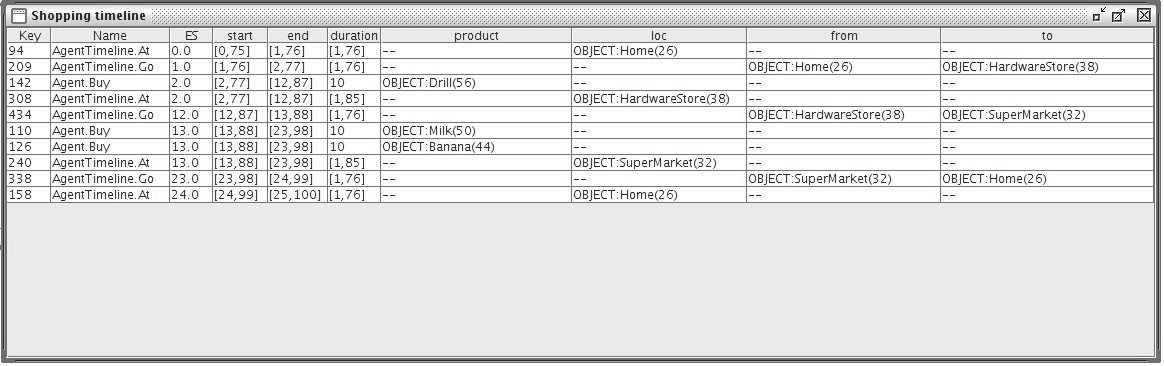
\includegraphics[scale=0.3]{figs/Example-Shopping0.jpg}
\caption{\small A \eu solution to a shopping agent problem domain where
  the agent needs to buy Bananas, Milk and a Drill.}
\label{fig:shopping-1}
\end{figure}

As the examples above show, a Planning problem (actions to achieve a
goal) may embed a Scheduling problem (what resources are necessary to
achieve stated goals) and both Planning and Scheduling may embed a
Constraint Satisfaction problem.  The relationships between Planning,
Scheduling and Constraint Satisfaction have been examined
\cite{smith00} and have lead to use of constraint reasoning in \eu as
a core building block.

\subsection{Constraint Programming}
\label{sec:europa:cp}

Constraint Satisfaction Programming (also known as Constraint
Programming or \textsf{CP}) is a discipline that provides a generic
framework for representing, solving and making logical inference on
constraints. A complete treatment of this discipline is given in
\cite{marriott98,apt03} with concise introductions provided in
\cite{bartak99,lustig01}.

A constraint programming problem consists of a set of variables $V=
{x_1,..,x_N}$, where each variable takes values from a domain
$d_1,..,d_N$; in this chapter we will deal only with discrete and
finite domains. Given a defined conjunctive set of constraints on the
variables: $C=\{c_1(x_1,..,x_N), ..., c_K(x_1,..,x_N)\}$, the
objective is to find one or more value assignments to $V$ where all
constraints are satisfied. To solve a problem, \textsf{CP} techniques
use logical inference to perform Constraint Propagation, which
consists of two operations:

\begin{enumerate}

\item \textbf{Bounds propagation} infers upper and lower variable
  bounds. For example, from the constraints $x_1 + x_2 \leq 2$ \& $x_i
  \geq 0$, we can infer $[0,2]$ bounds for $x_1$ and $x_2$.

\item \textbf{Domain reduction} infers a valid set of values for a
  variable.  For example, for constraints allDifferent($x_1,x_2,x_3$),
  $x_i \geq 0$ \& $x_i \leq 4$, if $x_1 = 1$ and $x_2 = 3$ we can
  infer that the valid and reduced domain for $x_3$ is $\{2,4\}$.

\end{enumerate}

A set of constraints and variables that describe a problem domain are
typically represented as a \emph{Constraint Network}, where the
variables are nodes and constraints are arcs between the variables. A
pair of variables $x \& y$ is said to be \emph{arc consistent} if for
every value in $x$'s domain, there is a value in $y$'s domain that is
consistent with all the constraints that connect $x$ and $y$.  A naive
approach to ensuring arc consistency consists of cycling through all
the variable pairs and performing constraint propagation until there
are no variable domain changes. The \texttt{AC-3} algorithm
\cite{mackworth77}, a popular implementation, improves over the naive
approach by ignoring constraints whose variables were not affected
since the last iteration. Fig. \ref{fig:constraintnet} shows a set of
constraints on $3$ variables ($x$, $y$ and $z$) represented as a
constraint network, and their domains before arc consistency is
enforced.  After the \texttt{AC-3} algorithm is executed, the domains
for the variables would be pruned to x=$\{2$\}, y=$\{2$\}, z=$\{2$\}.

\begin{figure}[!t]
\centering
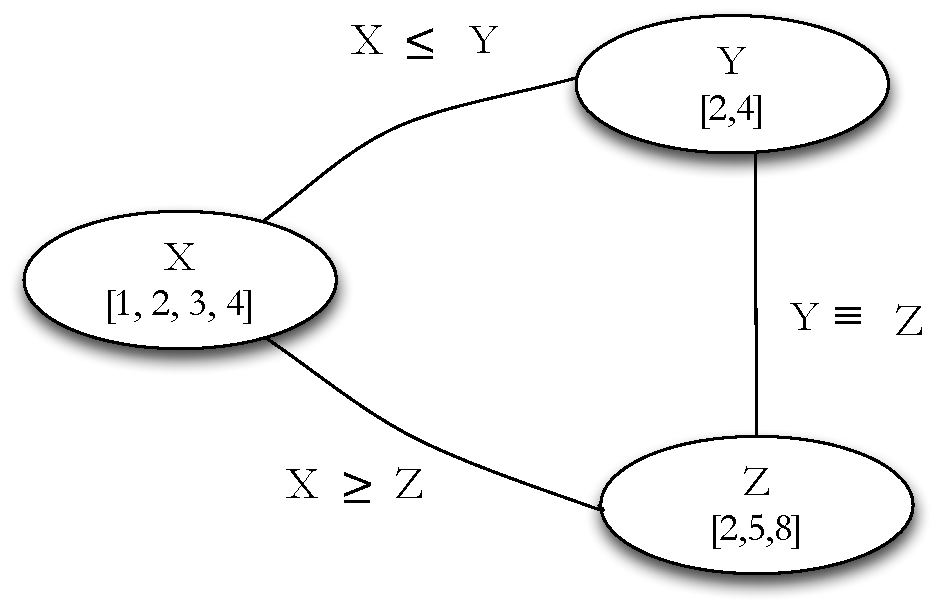
\includegraphics[scale=0.3]{figs/constraint-net.pdf}
\caption{\small Variables and Constraints represented as a Constraint Network}
\label{fig:constraintnet}
\end{figure}

Arc Consistency and other more stringent consistency definitions can
be used to efficiently prove that a \textsf{CP} problem is
unsatisfiable. However, they generally cannot prove that a \textsf{CP}
problem is satisfiable and provide specific variable assignments that
constitute solutions. To do so, search algorithms like global
backtracking \cite{hooker05} or local search are used; these use
consistency as an efficient way to prune the search space
\cite{cp06}. In theory, solving a \textsf{CP} problem is NP-Hard
\cite{ghallab04}, but often in practice a number of consistency and
search algorithms can be used.

\textsf{CP} is usually implemented as part of a programming language
and constraints are usually represented as objects \cite{puget95}. Any
constraint that the user is able to reason about can be introduced
into the system and, as long as the constraint propagation protocols
specified by the host \textsf{CP} system are enforced, it will be
indistinguishable from any other "primitive'' \textsf{CP} constraint,
such as $\leq$ or $\geq$.

\subsection{Constraint-Based Planning}
\label{sec:europa:cp}

The most common planning formulations use a propositional
representation, where the state of the world is represented by a set
of propositions (statements that can be true or false), and operators
change the truth values of these propositions \cite{gen87}. Although
these formulations are powerful and have allowed researchers to
develop numerous contributions in automated planning, there are many
classes of problem domains that are difficult to represent using this
formalism. In particular, it is hard to represent time, resources,
mutual exclusion and concurrency using propositions \cite{ghallab04}.
Constraint Programming is a framework that lends itself well to
represent and reason about all of those elements \cite{ghallab94}.
Consequently, there has been substantial effort in building automated
planners that take advantage of \textsf{CP} techniques.  The most
common approach in constraint-based planning has been to encode the
entire planning problem as a \textsf{CP} problem, where action choices
and relationships are represented as variables and/or constraints
\cite{do01,vanbeek99,vossen99,wolfman99}.  The advantage of using a
pure \textsf{CP} formulation is that standard solvers can be then used
to solve the planning problem. However, this approach also has a
couple of significant drawbacks:

\begin{enumerate} 

\item Given that action choices and relationships (rules) are
  expressed through variables, the domain descriptions that result
  from this approach are not intuitive and therefore difficult to
  understand and debug.

\item If the structure of a planning model (actions, conditions,
  effects, dependencies at the action level) is not explicitly
  maintained by the \textsf{CP} planner, the search algorithms are deprived of
  critical information to make better decisions. If that structure is
  maintained (for instance, by internally marking variables that
  represent action choice and relationships between actions), it is
  still hard to write search algorithms as any planning-specific
  insight has to be translated into the \textsf{CP} representation of
  variables and constraints.
  
\end{enumerate}

These drawbacks have been addressed by a number of planning frameworks
like \texttt{Descartes} \cite{joslin95,joslin96}, \texttt{IxTet}
\cite{ghallab87,lemai04} and \texttt{CAIP} (Constraint-Based Interval
and Attribute Planning) \cite{mus94,frank2003}.  These frameworks take
advantage of a \textsf{CP} representation to deal with time and resources, at
the same time maintaining an explicit representation of the elements
relevant to planning (action choices, causal relationships, etc). This
combination results in a planning approach that can deal with the type
of constraints found in real-world problems while allowing for
intuitive problem descriptions and a natural way to express search
algorithms and heuristics. \eu is one such implementation of the
\texttt{CAIP} framework, in which planning problems are specified in
terms of:

\begin{enumerate}

\item \textbf{Intervals}: entities that have a temporal scope (that
  is, a beginning and an end in time) and a set of
  attributes. Intervals are used to represent actions and states in
  the planning domain.

\item \textbf{Variables and Constraints}: Variables represent Interval
  attributes and constraints enable a direct representation of
  temporal, resource and any other restrictions that a valid plan must
  comply with.

\item \textbf{Domain Configuration Rules}: This is an explicit
  representation of the conceptual relationships between actions and
  states in the problem domain, for instance, for a Shopping Agent to
  be able to purchase a product, it must be at a location where the
  product is available.

\end{enumerate}

To generate plans, the \texttt{CAIP} framework uses a plan-space search
approach \cite{ghallab04}, where a partial plan is evolved until all
open goals are achieved, and all inconsistencies are removed. The
specific search algorithm used by \eu will be covered in detail below.


%%% Local Variables: 
%%% mode: latex
%%% TeX-master: "setobook"
%%% End: 
